\documentclass{article}
\usepackage{amsmath}
\usepackage{empheq}
\usepackage{graphicx}
\begin{document}
\title{
\Huge\textbf{Discrete Assignment}\\
\Huge\textbf{EE1205} Signals and Systems\\
\date{}
}
\large\author{Praful Kesavadas\\EE23BTECH11049}
\maketitle

\textbf{Question 11.9.1.2:}
Write the first five terms of the sequence whose $n^{th}$ terms  $x(n) = \frac{n}{n+1}$\\
\textbf{Solution:}
\begin{table}[ht]
    \centering
    \begin{tabular}{|c|c|c|}
    \hline
    \textbf{Term} & \textbf{Value} & \textbf{Description}\\
    \hline
    $x(0)$ & - & First term\\
    \hline
    $d$ & - & Common Difference\\
    \hline
    $x(n-1)$ & $x(0)+(n-1)d$ & General term\\
    \hline
    $x(p-1)$ & $a$ & pth term\\
    \hline
    $x(q-1)$ & $b$ & qth term\\
    \hline
    $x(r-1)$ & $c$ & rth term\\
    \hline
  \end{tabular}
  

    \caption{Variable description}
    \label{tab:11.9.1.2.1}
\end{table}\\
Z-transform is defined as, 

$$ x(n) \xleftrightarrow z  X(z)$$

\begin{align}
X(z) =  \sum_{i=-\infty}^\infty\ x(n).z^{-n}\
\end{align}
Here, Z-transform
\begin{align}
X(z) = \sum_{i=1}^\infty\ x(n).z^{-n}
\end{align}
\begin{align}
= \sum_{i=1}^\infty \frac{n}{n+1} . z^{-n}
\end{align}
On solving, 
\begin{align}
X(z) = \frac{1}{1-z^{-1}} + z\log{(1-z^{-1})}\
\end{align}
\begin{figure}[h]
    \centering
    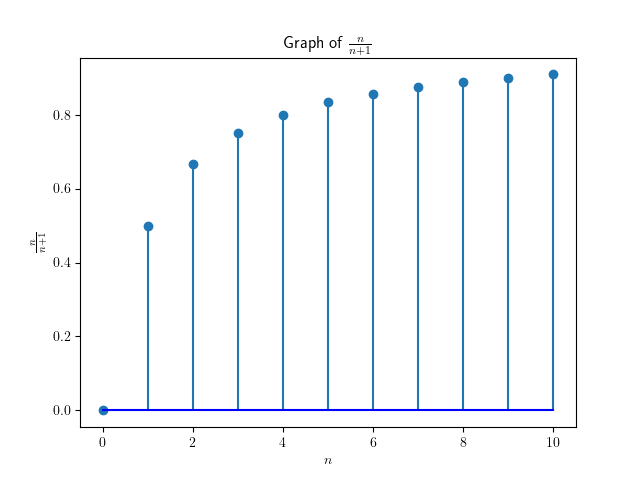
\includegraphics[width=0.7\linewidth]{figs/graph.png}
    \caption{Sequence plot generated from Python script}
    \label{fig:sequence-plot}
\end{figure}
\end{document}
